\documentclass[11pt,a4paper]{article}

\usepackage[english]{babel}
\usepackage[T1]{fontenc}
\usepackage[utf8]{inputenc}
\usepackage{graphicx}
\graphicspath{{../Figs/}}
\usepackage{float}
\usepackage{subcaption}
\usepackage[font=footnotesize,labelfont={sf,bf},textfont=sf,width=\textwidth]{caption}
\usepackage[margin=2cm]{geometry}
\usepackage[plainpages=false,pdfpagelabels,hypertexnames=false]{hyperref}
\usepackage[usenames,dvipsnames]{xcolor}
\usepackage{mathtools}
\usepackage[separate-uncertainty=true]{siunitx}
\usepackage{booktabs}
\usepackage{physics}


\title{\bfseries\textsc{Holography}}
\author{
Michele Masini\\ \small\texttt{\href{mailto:michele.masini@uni-ulm.de}{michele.masini@uni-ulm.de}}\and
Iyán Méndez Veiga\\ \small\texttt{\href{mailto:iyan.mendez-veiga@uni-ulm.de}{iyan.mendez-veiga@uni-ulm.de}}
}
\date{\today}


\begin{document}
\maketitle

\begin{abstract}
In this experiment we created four holograms. Holography is briefly explained theoretically and the experimental setup and procedures are described in detail. Pictures of the obtained holograms are shown, as well as results from two holographic interferometry measurements.
\end{abstract}

\vspace{1.5cm}

\section{Introduction}
In conventional imaging techniques, such as photography, what is recorded is merely the intensity distribution in the original scene. As a result, all information about the optical paths to different parts of the scene is lost.

The unique characteristic of holography is the idea of recording both the phase and the amplitude of the light waves from an object but since all recording materials respond only to the intensity in the image, it is necessary to convert
the phase information into variations of intensity.

The purpose of this report is to show, both theoretical and experimentally, how this can be achieved using coherent light.

We will start from the very beginning and the foundation of classical electromagnetism: the Maxwell equations. Then, we will describe how EM fields propagate by derivating the wave equation from the Maxwell equations and write some of its solutions. We will also see the implications of the superposition principle and what we mean by coherent light. A brief summary of the physics of lasers will be presented and, finally, holography will be explained. Additionally, we will describe the experimental procedure to create the holograms, and at the end we will show the obtained holograms.


\section{Theory}

\subsection{Maxwell equations}
Maxwell equations \cite{feynman} are a set of linear differential equations that describe how electric and magnetic fields are generated by charges, currents, and changes of the fields. Together with the Lorentz force, $\vb{F}=q(\vb{E}+\vb{v}\times\vb{B})$, form the foundation of classical electromagnetism.

The complete Maxwell equations are the following:

\begin{subequations}\label{eq:maxwell_equations}
\begin{align}
&\div\vb{E}=\frac{\rho}{\epsilon_0}\label{eq:maxwell_1}\\
&\curl\vb{E}=-\pdv{\vb{B}}{t}\label{eq:maxwell_2}\\
&\div\vb{B}=0\label{eq:maxwell_3}\\
&\curl\vb{B}=\frac{1}{c^2}\qty(\frac{\vb{j}}{\epsilon_0}+\pdv{\vb{E}}{t})\label{eq:maxwell_4}
\end{align}
\end{subequations}

The first equation \eqref{eq:maxwell_1}, read as \emph{the divergence of $\vb*{E}$ is the charge density over $\epsilon_0$}, is the differential form of the Gauss' law, which is always valid both in dynamic and static fields. Equivalently, in the integral form it means that the flux of the electric field through a closed surface is equal to the charge inside that surface over the vacuum permittivity, i.e. the capability of the vacuum to permit electric field lines.

The third equation \eqref{eq:maxwell_3} is the corresponding general law for magnetic fields. That the divergence of the magnetic field is zero is the mathematical way of expressing that magnetic monopoles cannot be found in nature.

The second equation \eqref{eq:maxwell_2}, that \emph{the curl of $\vb*{E}$ is -$\pdv*{\vb*{B}}{t}$}, is the differential form of the Faraday's law. The line integral of the electric field around a loop is equal to minus the derivative with respect to time of the flux of the magnetic field through that loop.

Last equation \eqref{eq:maxwell_4}, when Maxwell wrote it down, included new physics. He added a new term when he noticed something strange in the expression that was used before to explain magnetic fields produced by steady currents $\curl\vb{B}=\vb{j}/(c^2\epsilon_0$). Taking the divergence on both sides, the left-hand side is zero\footnote{The divergence of a curl is always zero.}, and if we want the equation to be true then we require that the divergence of $\vb{j}$ is also zero. This means that the total flux of current out of any closed surface has to be zero, and this makes no sense since we know that charges can move from one place to another. Maxwell's solution was to add the extra term $\pdv*{\vb{E}}{t}$ to the right-hand side, which became his fourth and last equation.

In the integral form, we can read the fourth equation as: the integral of the magnetic field around a loop is proportional, being the proportionality constant one over the speed of light squared, to the current through the loop over the vacuum permittivity plus the derivative with respect to time of the flux of the electric field that goes through the same loop.

If we accept Maxwell's equations, and we should since no one has ever found an experiment that disagrees with them, we must conclude that charge is always conserved. Conversely, if we assume that the electric charge is conserved, and we write this fundamental law as $\div\vb{j}=-\pdv*{\rho}{t}$, meaning that any flow of charge must come from some supply, then this is exactly the term that Maxwell had to add to straighten out the difficulty we found.

\subsection{Wave equation (Michele)}
What you did in the colloquium and put some solutions (plane and spherical waves, and Gaussian beams for example)

By means of the Maxwell equations, it is possible to describe the propagation of light as the propagation of a wave called electromagnetic wave. It is not hard to imagine that light does not carry charge, hence we will suppose $\rho=0$ and $\textbf{j}=0$.

In this conditions, Maxwell's equations read:
\begin{subequations}\label{eq:maxwell_equations_wo_charge}
\begin{align}
&\div\vb{E}=0\label{eq:maxwell__wo_1}\\
&\curl\vb{E}=-\pdv{\vb{B}}{t}\label{eq:maxwell_wo_2}\\
&\div\vb{B}=0\label{eq:maxwell_wo_3}\\
&\curl\vb{B}=\frac{1}{c^2}\qty(\pdv{\vb{E}}{t})\label{eq:maxwell_wo_4}
\end{align}
\end{subequations}

We can decouple the previous equations using the following rule:
\begin{equation}
\curl \curl \vb{F}=\nabla (\div \vb{F})- \nabla^2\vb{F}\label{rule}
\end{equation}
where $\vb{F}$ is a generic field. Let us apply for instance equation (\ref{eq:maxwell_wo_3}) and (\ref{eq:maxwell_wo_4}) to (\ref{rule}) to get:
\begin{align*}
\curl \curl \vb{B} &=\nabla (\div \vb{B})- \nabla^2\vb{B} \\
\curl \frac{1}{c^2}\qty(\pdv{\vb{E}}{t}) &=0-\nabla^2\vb{B} \\
\frac{1}{c^2}\qty(\pdv{\curl \vb{E}}{t}) &=-\nabla^2\vb{B}
\end{align*}
Finally, using (\ref{eq:maxwell_wo_2}):
\begin{equation}
\nabla^2\vb{B}=\frac{1}{c^2}\pdv{^2 \vb{B}}{t^2}
\end{equation}
Analogously for the electric field, we obtain:
\begin{equation}
\nabla^2\vb{E}=\frac{1}{c^2}\pdv{^2 \vb{E}}{t^2}
\end{equation}
We have obtained two three-dimensional wave equations. The general solution is of the form:
\begin{align}
\vb{B}(\vb{r},t) &=\vb{B_0}e^{i(\vb{k} \cdot \vb{r}-\omega t+\phi_0)}\\
\vb{E}(\vb{r},t) &=\vb{E_0}e^{i(\vb{k} \cdot \vb{r}-\omega t+\phi_0)}\label{elec}
\end{align}
If we suppose that the wave is propagating only along z, we have:
\begin{align}
\vb{B}(z,t) &=\vb{B_0}e^{i(kz-\omega t+\phi_0)}\\
\vb{E}(z,t) &=\vb{E_0}e^{i(kz-\omega t+\phi_0)}
\end{align}
Using equation (\ref{eq:maxwell__wo_1}) and (\ref{eq:maxwell_wo_3}), we can see that the z-component of the fields is zero. Moreover, using equation (\ref{eq:maxwell_wo_2}), we easily notice that magnetic and electric field have to be orthogonal.
\subsection{Superposition principle (Michele)}
What you explained in the colloquium but don't forget to mention that the reason for this is because Maxwell equations are linear.

Let us suppose that we have 2 waves of the form (\ref{elec})\footnote{We call $\phi_{1,2}(t)\equiv\vb{k_{1,2}} \cdot \vb{r}-\omega_{1,2} t+\phi_0$}. We will see what an observer would measure looking at the superposition between the two waves. What we are going to measure in a laboratory is the intensity of light, where $I\propto \abs{\vb{E}}^2$.

In our case:
\begin{align*}
I_{TOT}\propto \abs{\vb{E_1}+\vb{E_2}}^2 &=\abs{\vb{E_{0,1}}e^{i\phi_1}+\vb{E_{0,2}}e^{i\phi_2(t)}}^2\\
&=\abs{\vb{E_{0,1}}}^2+\abs{\vb{E_{0,2}}}^2+\vb{E_{0,1}}\cdot \vb{E_{0,2}}e^{i\phi_1}e^{-i\phi_2(t)}+\vb{E_{0,2}}\cdot \vb{E_{0,1}}e^{i\phi_2(t)}e^{-i\phi_1(t)}
\end{align*}
Finally, using Euler's formulae we get:
\begin{equation}
I_{TOT}(t)\propto I_1+I_2+2\vb{E_{0,1}}\cdot \vb{E_{0,2}}cos(\phi_1(t)-\phi_2(t))
\end{equation}
We can notice that there is a superposition term in the result. This term is responsible of the so called \emph{interference}, i.e. constructive (when $cos(\Delta\phi)>0$) or distructive (when $cos(\Delta\phi)<0$) superposition of the two waves.  Anyway, it is really hard to observe this term because, during an experiment, we measure the avarage of the intensity over a certain interval of time:
\begin{align*}
I_{AV} &= \frac{1}{t_{max}}\int_0^{t_{max}}I(t)dt\\ &\propto I_1+I_2+ 2\vb{E_{0,1}}\cdot \vb{E_{0,2}} \frac{1}{t_{max}} \int_0^{t_{max}} cos(\phi_1(\vb{r},t)-\phi_2(\vb{r},t)) dt\xrightarrow{t_{max}\rightarrow \infty} I_1+I_2
\end{align*}


\subsection{Coherence (Michele)}
When we speak about \emph{coherence of light}, we are referring to two or more waves whose phase difference $\Delta\phi(\vb{r},t)\equiv \phi_1(\vb{r},t)-\phi_2(\vb{r},t)$ is constant in space and time:
\begin{equation}
\Delta\phi(\vb{r},t)=\Delta\phi_0
\end{equation}
A second reason why we do not observe interference in everyday life is the fact that the superposition term varies too fastly because of the non-coherence of light coming from natural sources.

We will introduce 2 kinds of coherence: temporal and spatial coherence. We speak about the former when we start with 2 equal waves, we introduce a retardation in one of them (let us say $\tau_0$) and we observe their superposition. We will have a phenomenon of interference due to their pase difference $\omega \tau_0$ and we will call \emph{coherence lenght} the difference of optical path between the 2 waves: $l_c\equiv c\tau_0$.

As far as spatial coherence is concerned, it arises when 2 fields arrive in 2 different points of space. This will cause a phase difference.

\subsection{Physics of lasers (Iyán)}

\subsection{Holography (together?)}

\begin{figure}[ht]
\centering
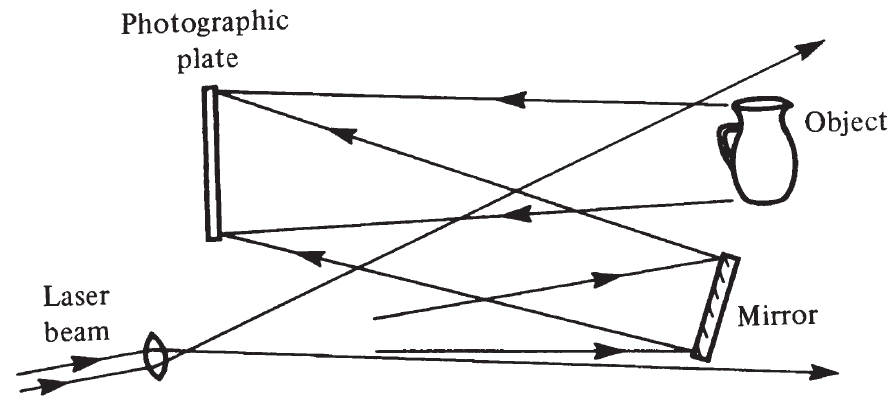
\includegraphics[width=0.8\textwidth]{Hologram_recording}
\caption{Diagram of the hologram recording setup. The interference pattern produced by the reference wave and the object wave is recorded.\cite{hariharan_2002}}
\label{fig:hologram_recording}
\end{figure}

\begin{figure}[ht]
\centering
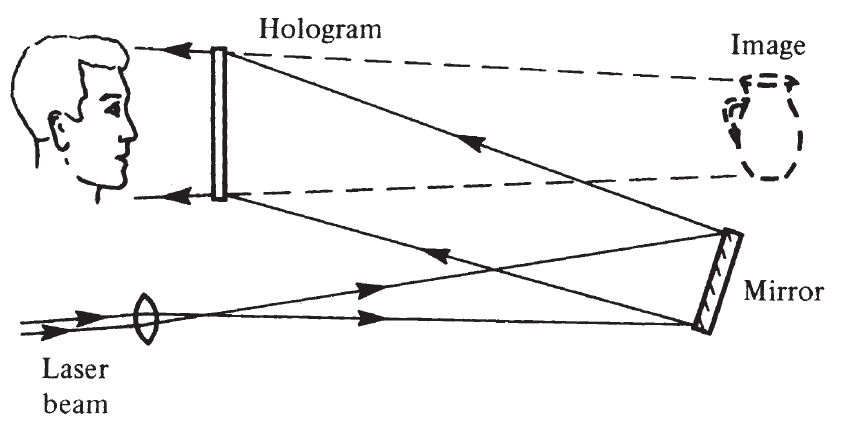
\includegraphics[width=0.8\textwidth]{Hologram_image_reconstruction}
\caption{Diagram of the image reconstruction. Light diffracted by the hologram reconstructs the original object wave.\cite{hariharan_2002}}
\label{fig:hologram_reconstruction}
\end{figure}

\section{Experimental procedure}
\paragraph{Optical setup}
The first thing we had to do was adjust the optical bench. Almost everything was already set up but we did have to align the objective and the spatial filter for the reference beam. These optical elements are placed just after the beam splitter in the path of the reference beam (see Figure \ref{fig:optical_bench_1}). First we aligned the backside of the objective with the help of a small paper sheet. Then we put the spatial filter just after it and use the screws to align it at exactly where the beam was focused. Transversal alignment was done by trying to find the maximum of light through the spatial filter. Once we did that, we move the spatial filter in the longitudinal direction till the Airy pattern due to diffraction from the optical system's aperture disappeared and we had a clear Gaussian beam.

\begin{figure}[ht]
\centering
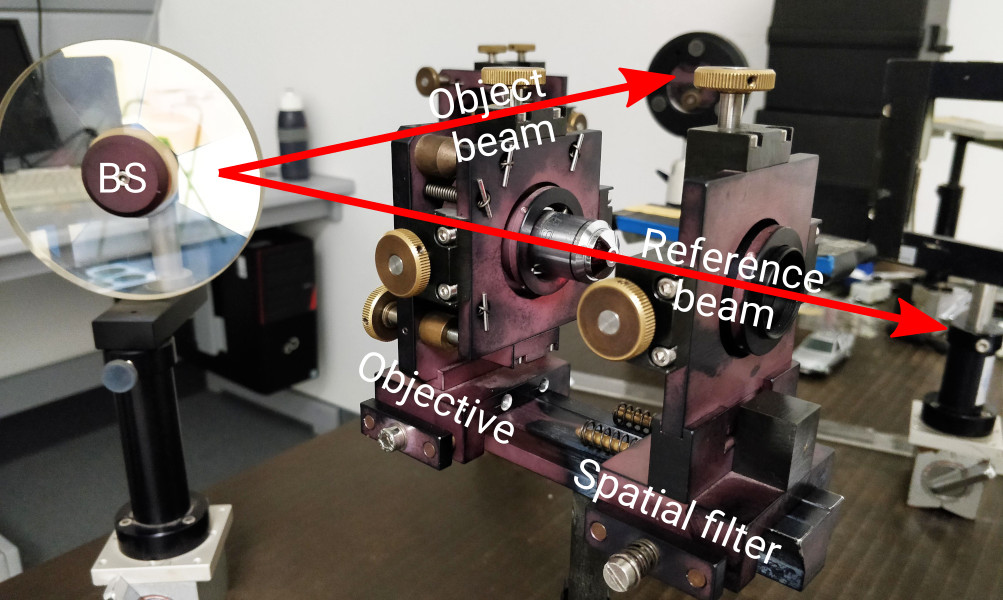
\includegraphics[width=0.8\textwidth]{Optical_bench_1}
\caption{The BS divides the laser in two beams: the reference and the object beam. Reference beam goes through an objective and a spatial filter in order to obtain a Gaussian beam, which is reflected by a mirror to the photosensitive plate.}
\label{fig:optical_bench_1}
\end{figure}

\paragraph{Mixing of chemicals}
In order to observe the hologram, we needed to protect the photosensitive material from light once we exposed it to the desired object. This was done by using a negative developer and a rapid fixer. We prepared two solutions using the the chemicals produced by \href{https://www.tetenal.com/}{Tetenal} shown in Figure \ref{fig:chemicals}. We prepared \SI{1}{\litre} of developer by mixing \SI{200}{\milli\litre} of the ultrafin with \SI{800}{\milli\litre} of water. We also prepared \SI{1}{\litre} of fixer with \SI{150}{\milli\litre} of the superfix plus and \SI{850}{\milli\litre} of water.

The procedure to expose, develop and fix the photosensitive plate was the following: \SI{90}{\second} of exposure to the object and reference beams, \SI{2}{\min} bath in the developer dilution, \SI{10}{\second} bath in water, \SI{4}{\min} bath in the fixer dilution, and finally \SI{2}{\min} bath in water. After this, the plates were put to dry next to a fan.

\begin{figure}[ht]
\centering
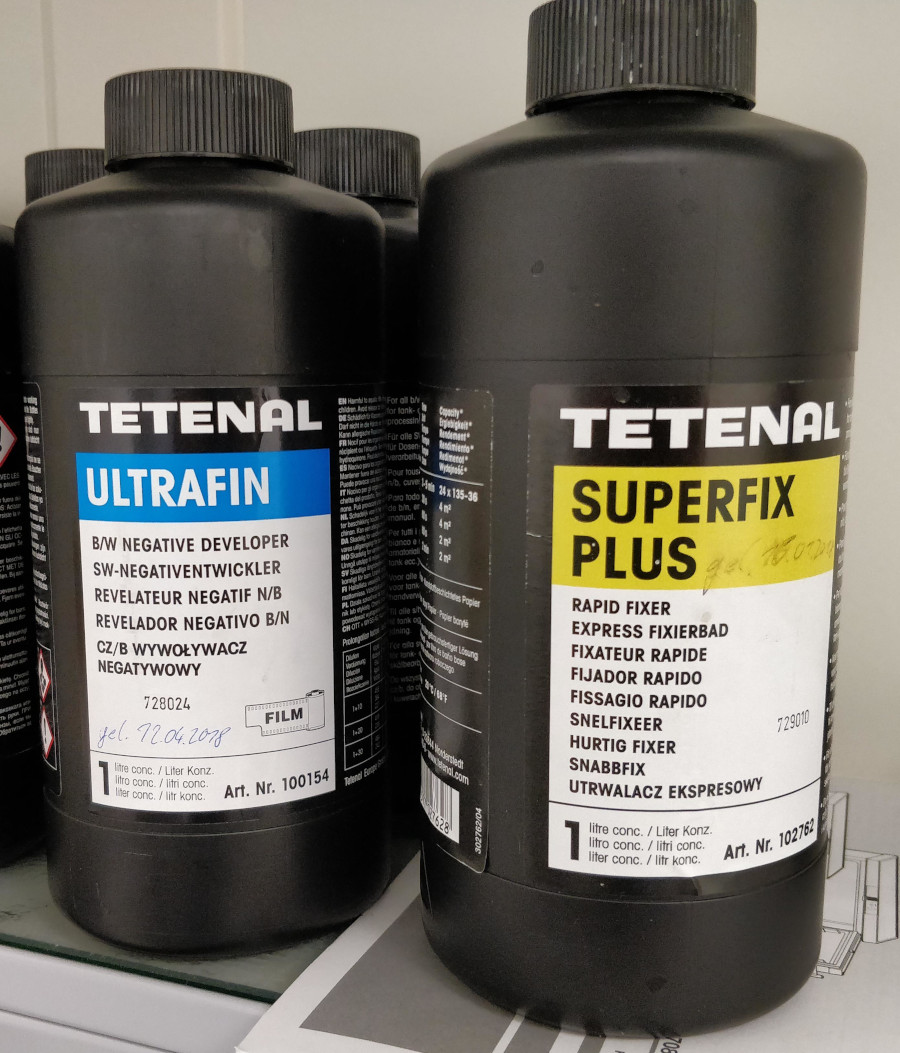
\includegraphics[width=0.3\textwidth]{Chemicals}
\caption{The negative developer and the rapid fixer used to prepare the two dilutions.}
\label{fig:chemicals}
\end{figure}

\paragraph{Hologram creation}
An object is illuminated by the object beam and the reflected light reaches the photosensitive plate. Simultaneously, the reference beam illuminates directly the photosensitive plate in order to obtain an interference pattern. {\color{red}Complete when formulas are written in the Theory section.} For creating the hologram, the beam splitter is put in the 95-5 position, so 5\% of the intensity of the light goes to the reference path and 95\% illuminates the object.

\paragraph{Holography interferometry}
In order to see interference fringes in the hologram, instead of the long single \SI{90}{\second} exposure mentioned before, we used two \SI{45}{\second} exposures, and we moved the object, by either a very small distance or an angle, after the first exposure.

Number of fringes were obtained using \href{https://imagej.net/}{ImageJ}. Images were first desaturated and then the profile of a line crossing all the fringes was plotted. By counting the peaks we determined the number of fringes.


\section{Results and conclusions (Michele)}

\begin{figure}[ht]
\centering
\begin{subfigure}[b]{0.45\textwidth}
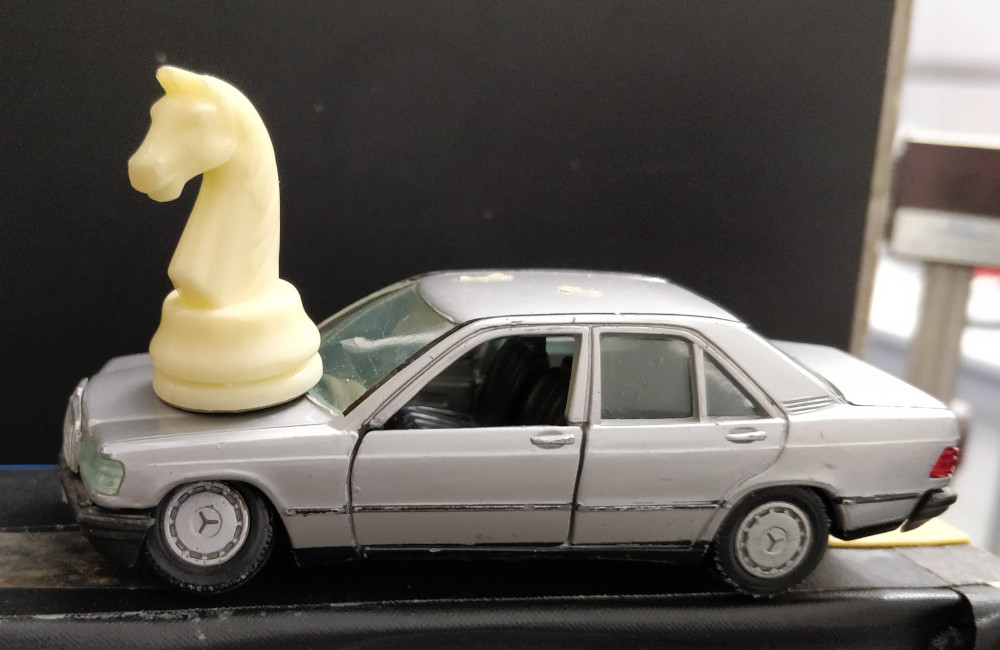
\includegraphics[width=\textwidth]{car_knight}
\caption{Object}
\label{fig:car_knight}
\end{subfigure}
\begin{subfigure}[b]{0.45\textwidth}
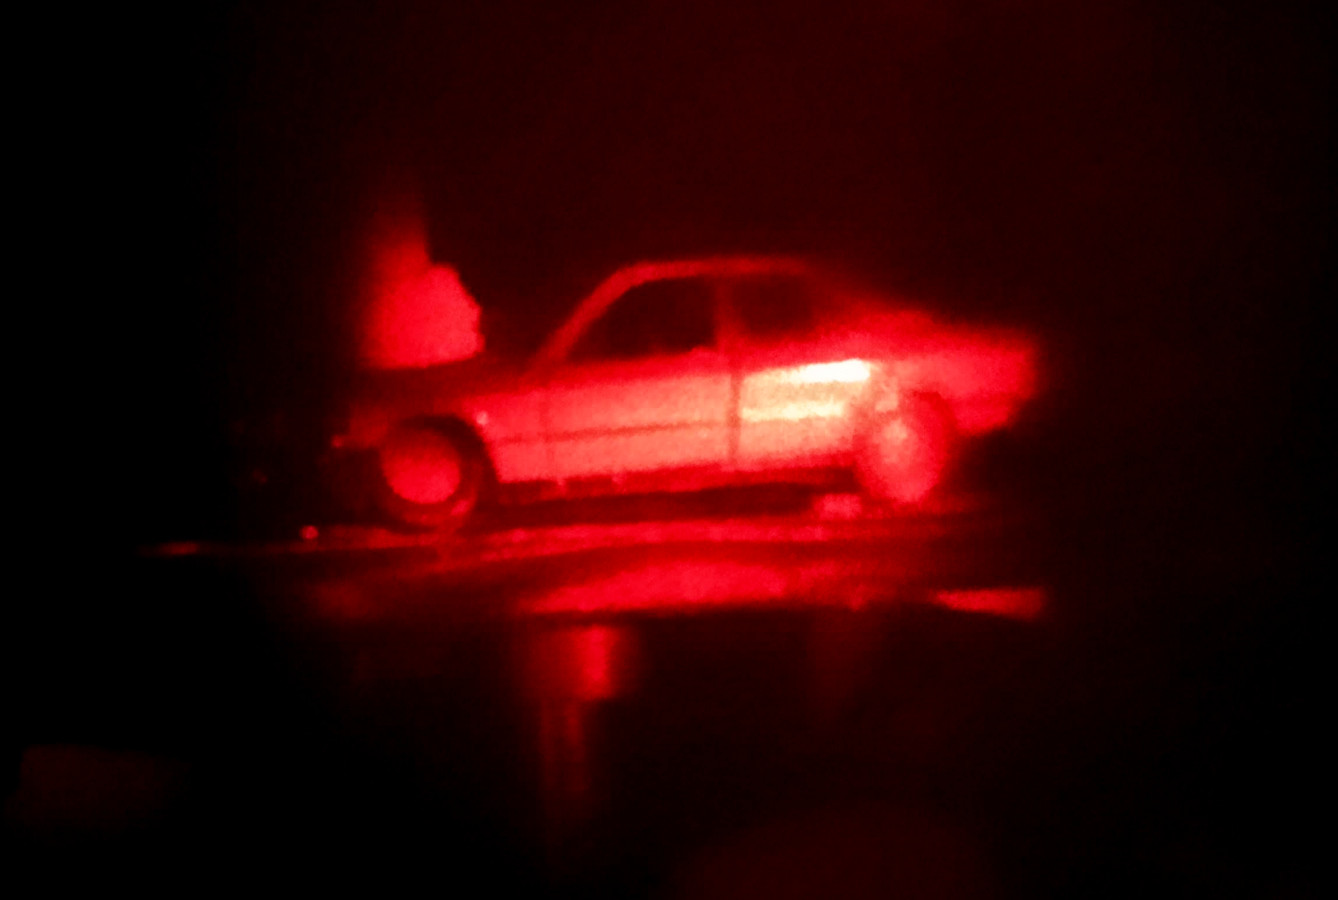
\includegraphics[width=\textwidth]{Off-axis_hologram}
\caption{Hologram}
\label{fig:off_axis_hologram}
\end{subfigure}
\caption{Off-axis exposure of a car with a knight chess piece on the bonnet. On the left, a picture of the original object. On the right, a picture of the obtained hologram.}
\label{fig:off-axis_exposure}
\end{figure}

\begin{figure}[ht]
\centering
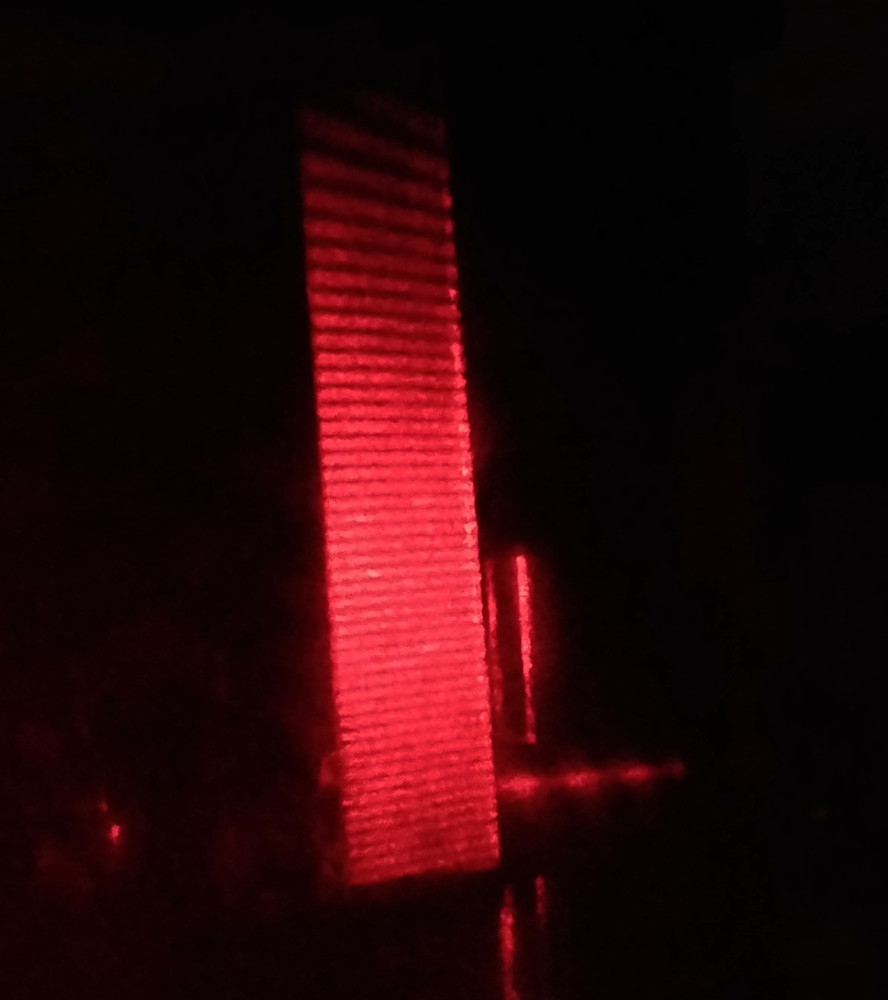
\includegraphics[width=0.6\textwidth]{Holographic_interferometry_position}
\caption{Picture of an hologram with an interference pattern caused by the movement of the metallic piece $\approx\SI{14}{\micro \m}$ between exposures.}
\label{fig:holographic_interferometry_position}
\end{figure}

\begin{figure}[ht]
\centering
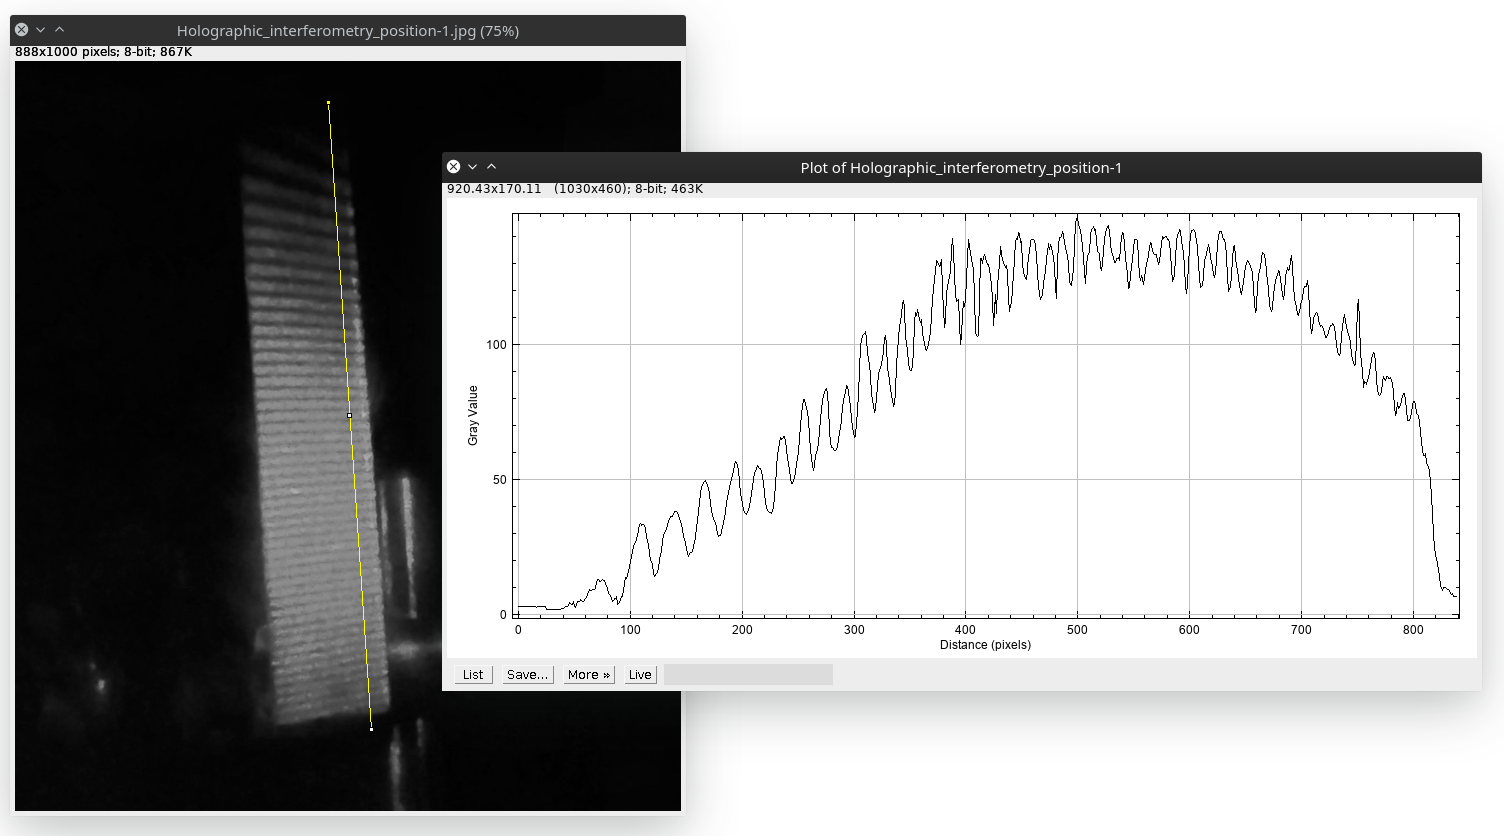
\includegraphics[width=\textwidth]{Holographic_interferometry_position_fringes}
\caption{Profile along the vertical direction (yellow line). Peaks correspond to constructive interference and by counting them we get the number of fringes.}
\label{fig:holographic_interferometry_position_fringes}
\end{figure}

\begin{figure}[ht]
\centering
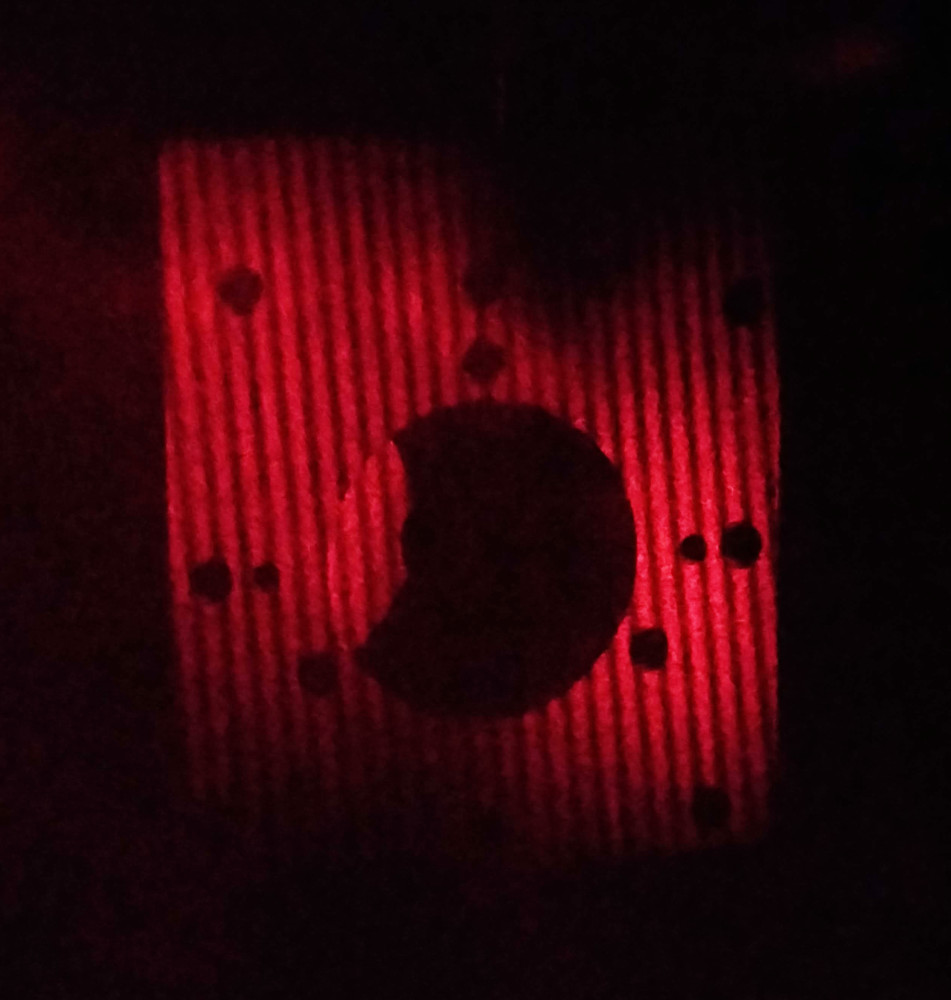
\includegraphics[width=0.6\textwidth]{Holographic_interferometry_angle}
\caption{Picture of an hologram with an interference pattern caused by the rotation of the metallic piece $\approx (1/72)^\circ$ between exposures.}
\label{fig:holographic_interferometry_angle}
\end{figure}

\begin{figure}[ht]
\centering
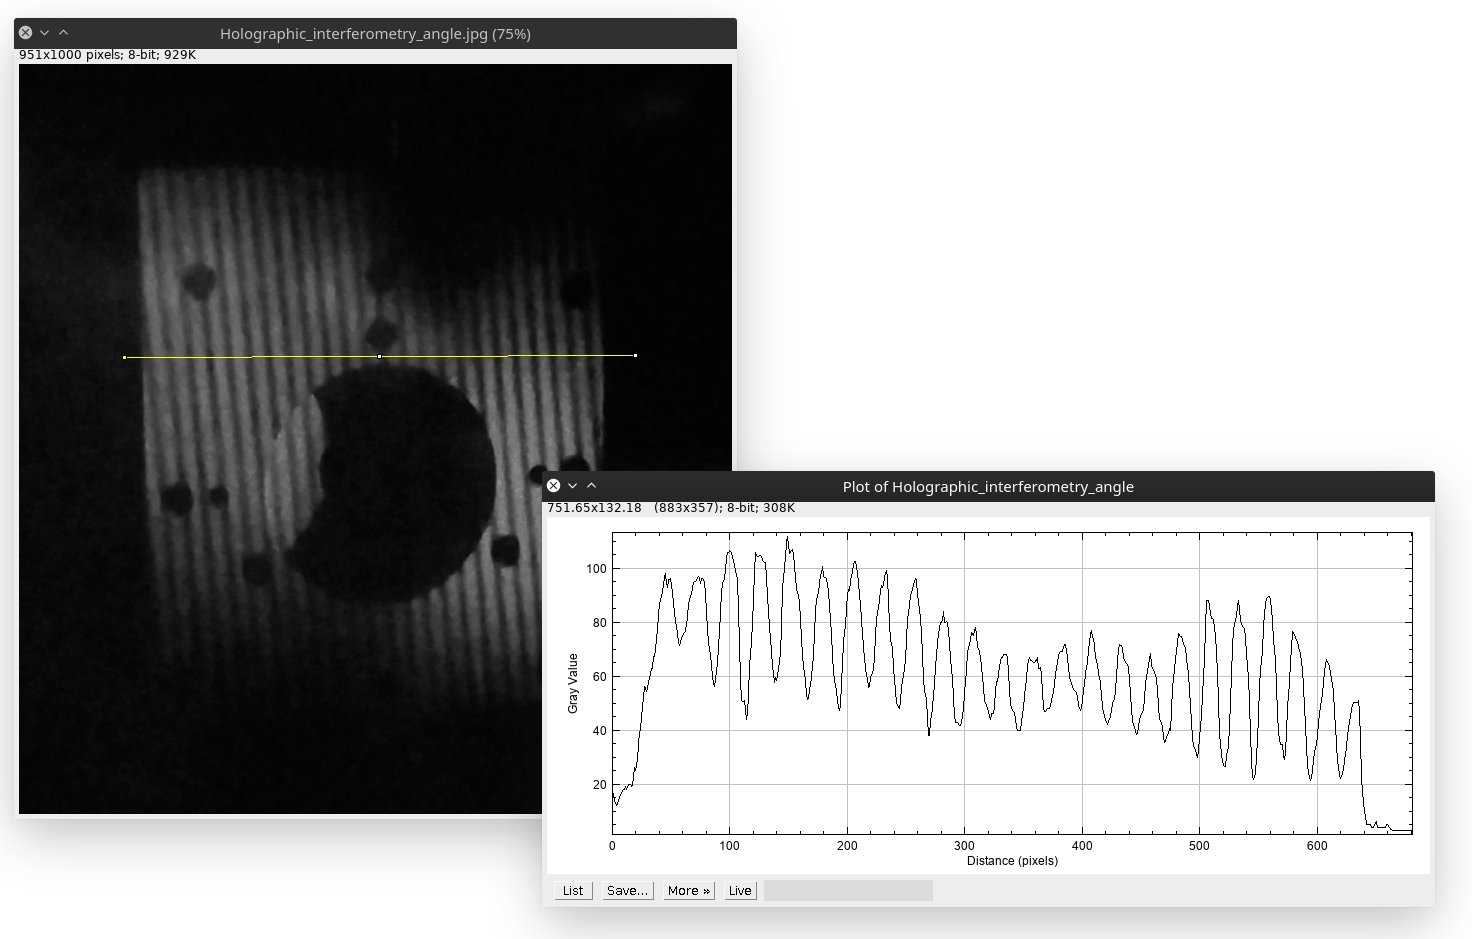
\includegraphics[width=\textwidth]{Holographic_interferometry_angle_fringes}
\caption{Profile along the horizontal direction (yellow line).}
\label{fig:holographic_interferometry_angle_fringes}
\end{figure}

\begin{figure}[ht]
\centering
\begin{subfigure}[b]{0.45\textwidth}
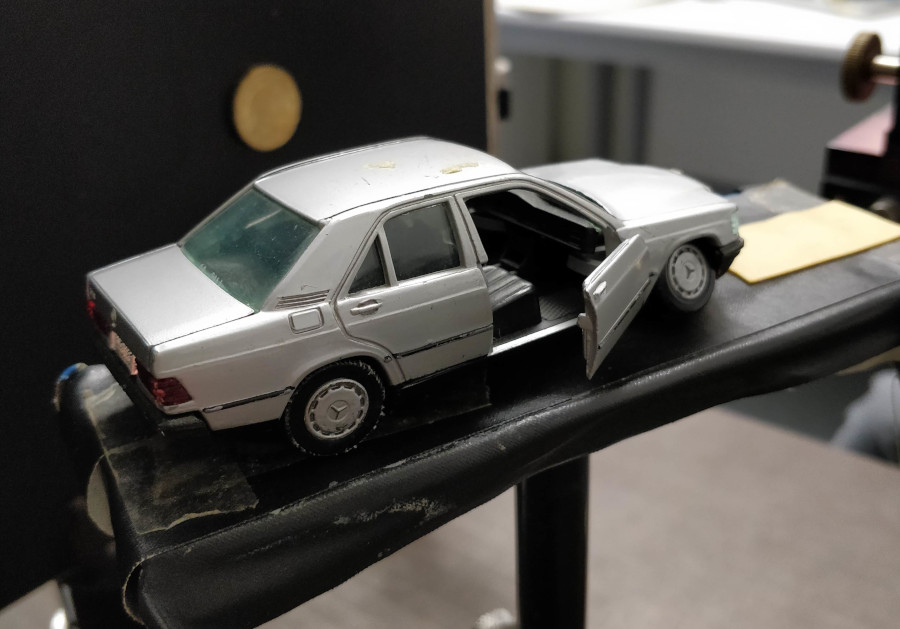
\includegraphics[width=\textwidth]{car_double_exposure_1}
\caption{Position first exposure}
\label{fig:car_knight}
\end{subfigure}
\begin{subfigure}[b]{0.45\textwidth}
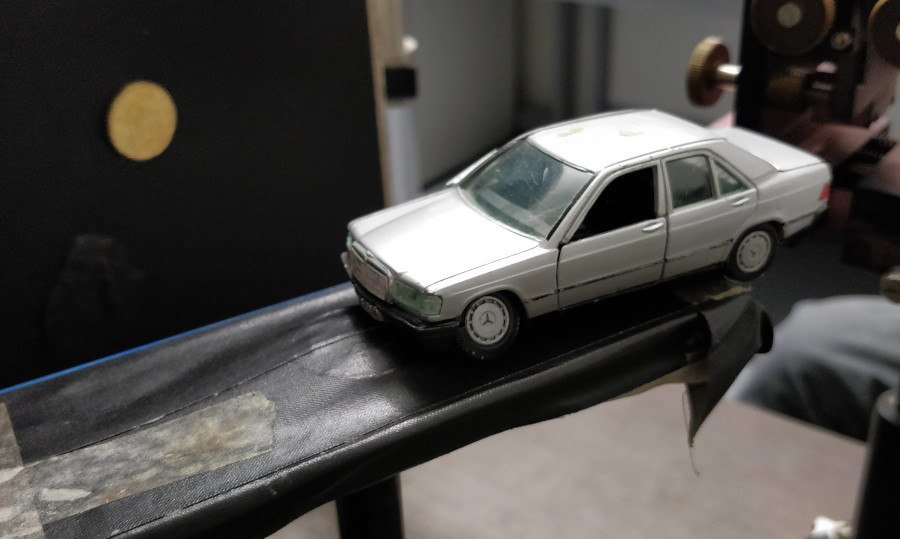
\includegraphics[width=\textwidth]{car_double_exposure_2}
\caption{Position second exposure}
\label{fig:off_axis_hologram}
\end{subfigure}\\\vspace{.2cm}
\begin{subfigure}[b]{0.45\textwidth}
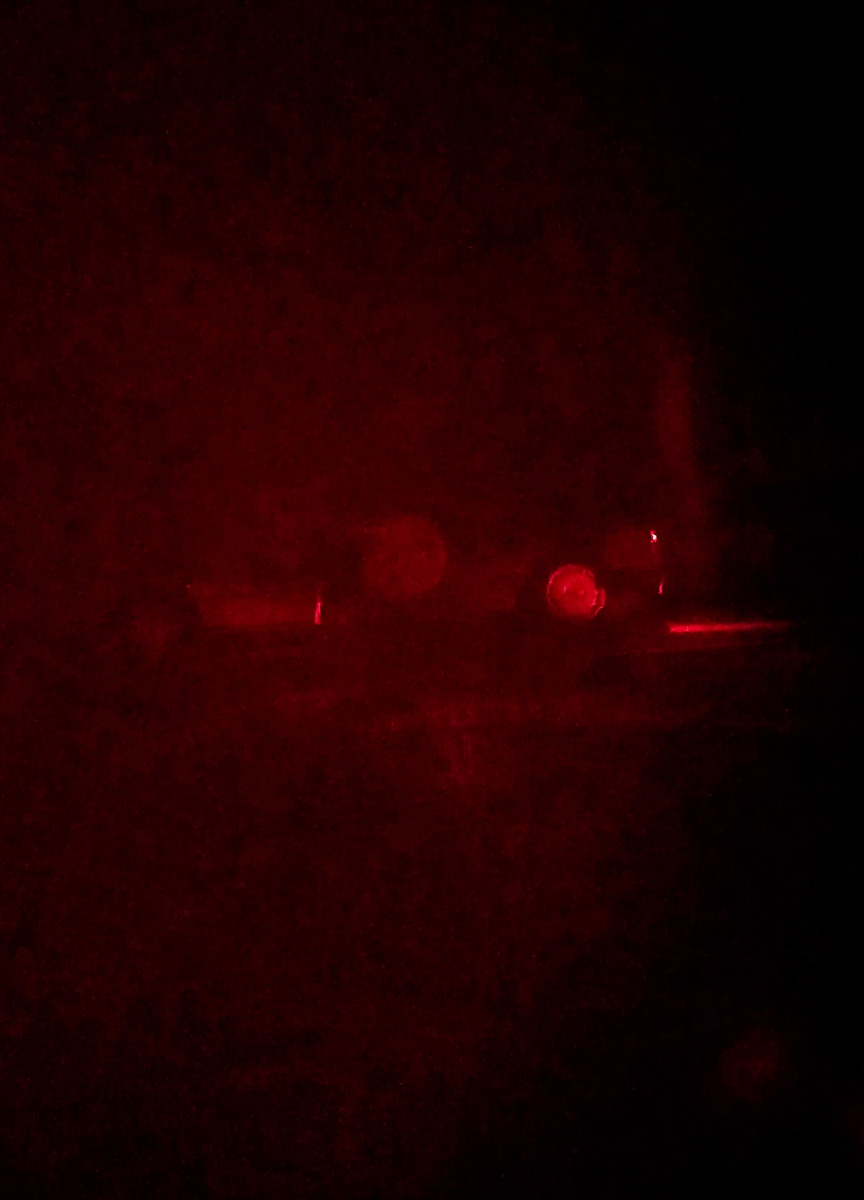
\includegraphics[width=\textwidth]{car_double_exposure_hologram}
\caption{Picture of the obtained hologram}
\label{fig:car_knight}
\end{subfigure}
\caption{Setup and hologram of a double \SI{45}{\second} exposure in which we moved and rotated the car between exposures.}
\label{fig:experiment_double_exposure}
\end{figure}

\nocite{*}
\bibliographystyle{unsrt}
\bibliography{references}
\end{document}